%!TEX root = thesis.tex

\chapter{Motion planning}
Chapter overview

\section{Introduction}
What means motion planning?
What are the requirements?


\section{The MoveIt! motion planning framework}

MoveIt\footnote{http://moveit.ros.org} is an open source framework for motion planning. It is the successor of the previous arm navigation stack and therefore fully integrated into ROS. MoveIt was originally developed by Willowgarage\footnote{http://www.willowgarage.com} but since April 2012 it is maintained by the Open Source Robotics Foundation (OSRF). Figure\ref{fig:moveit_arch} gives an overview about the system architecture. Central part of the framework is the \texttt{move\_group} node which  provides a rich set of ROS topics and services that can be used to solve planning problems and execute calculated motion plans on connected hardware. Configuration of that node happens via the parameter server. It requires a complete kinematic and semantic description of the robot setup and a lot of other configuration parameters which will be described in subsequent sections. The most important parts of MoveIt are implemented as plugins which means that it is highly customizable. By default it uses the Kinematics and Dynamics Library\footnote{http://www.orocos.org/kdl} (KDL) as IK solver and the Open Motion Planning Library (OMPL) as planning plugin but it is possible to replace them with custom solutions if necessary.\\

\begin{figure}[ht]
	\centering
  	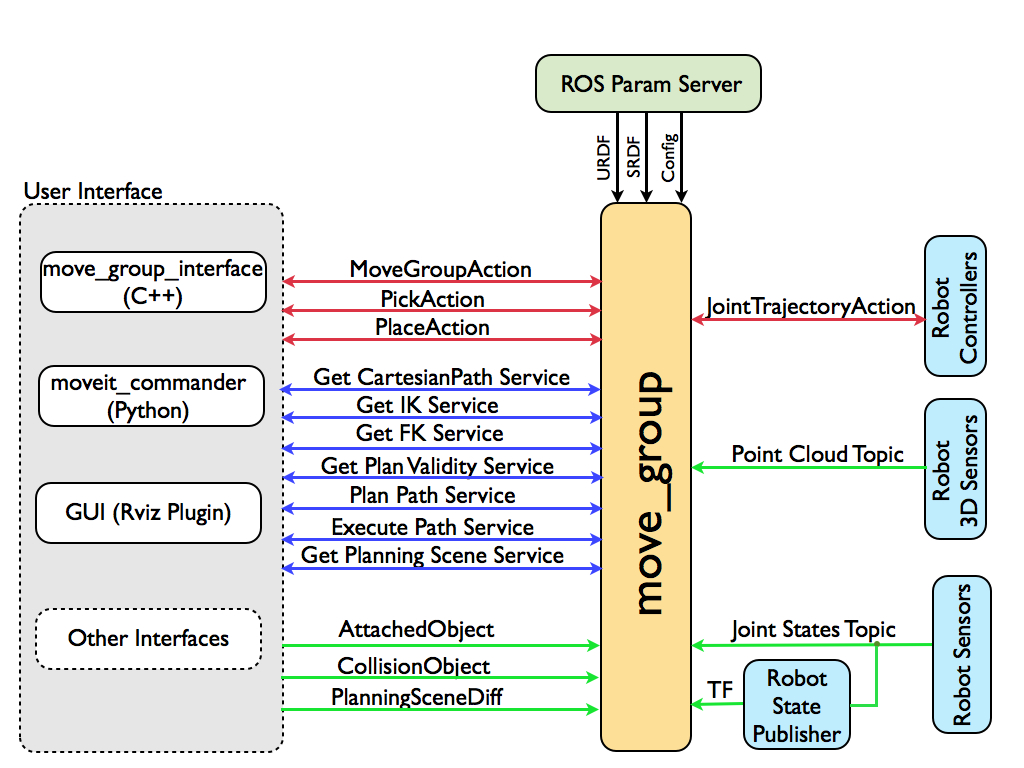
\includegraphics[width=0.75\textwidth]{images/moveit_architecture.jpg}
	\caption[Moveit architecture]{MoveIt architecture}
	{\scriptsize Image source: \url{http://moveit.ros.org/documentation/concepts}}
	\label{fig:moveit_arch}
\end{figure}

MoveIt maintains a planning scene which is an internal representation of the world, including the robot and it's environment. The base is a description of the robot and it's various planning groups. 
The kinematic description needs to be available in form of a URDF model. Necessary steps to create that model are described in Section\ref{sec:urdf}. Based on that URDF model, a semantic description (SRDF) is created that contains additional information about the setup, as explained in Section\ref{sec:moveit_assistant}. On top of those static descriptions, MoveIt allows to modify the planning scene on runtime via appropriate ROS topics.\\

To keep track of the current state of the robot MoveIt needs to be informed continuously about actual joint states. This is done via publishing the joint states to a specific topic. If there are additional objects within the robot's workspace they also have to be added to the planning scene. This can be done either by explicitly adding them via the corresponding topic or by integrating sensor information like Kinect camera data. MoveIt can then take those objects into account during motion planning and avoid collisions. But some collisions are intended. For example if an object has to be picked up, the gripper has to get in contact to this object. Therefore collision checking for specific objects can be (temporary) disabled to allow those controlled collisions. Therefore MoveIt maintains an \emph{AllowedCollisionMatrix} to which objects can be added or removed. The connection to the hardware happens via the \emph{FollowJointTrajectory} action interface. Each robot component has to provide this interface if it is intended to be control via MoveIt. This interface consists of a set of ROS topics that provide trajectory execution functionality and also allow monitoring the current execution status. The major contribution within this chapter to the whole project was to provide an implementation of this interface and connect it to the one that is currently available.

\section{Creating the URDF model of the robot setup}
\label{sec:urdf}

The \emph{Unified Robot Description Format} (URDF) is a markup language, designed to describe robots. The description happens in text files, in a special XML format. The most important elements in the XML specification\footnote{http://wiki.ros.org/urdf/XML} are:

\begin{itemize}

\item \textbf{<link>} \\
Describes the all necessary properties of a specific robot link. Each link must have a unique name. The visual, inertial and collision details are configured in the corresponding subtags of the link element. The visual part as well as the collision model can either be composed from primitive shapes
or from mesh files. If mesh files are used it is important that they are not to complex. Especially for the collision model it is recommended to use a simplified model to avoid a performance loss.

\item \textbf{<joint>} \\
Describes the properties of a joint. A joint is a connection between two links, having exactly one parent and one child link. Each joint states a new reference frame for it's child link and it is positioned relative to it's parent frame. A \emph{fixed} joint is a rigid connection between parent and child link. There are different types of joints available but for the current project only \emph{revolute} joints\footnote{Rotational joint with one degree of freedom} are of interest. Details like limits, axis orientation and dynamic properties can be configured in the corresponding subtags of the joint element.

\end{itemize}
\begin{figure}[ht]
	\centering
  	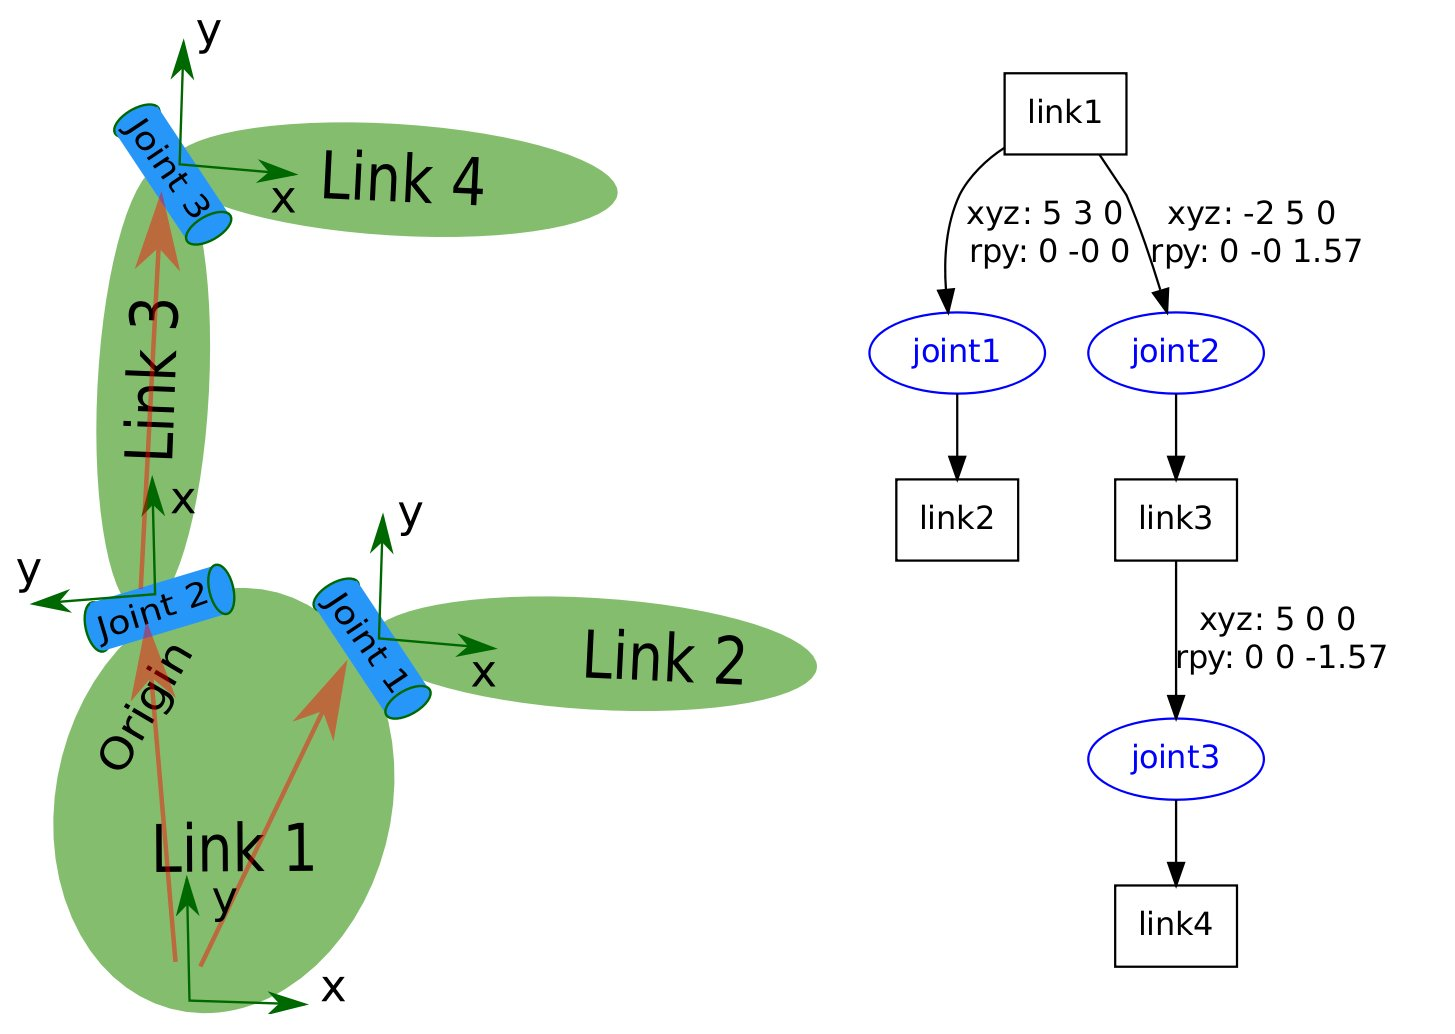
\includegraphics[width=0.75\textwidth]{images/urdf_chain.jpg}
	\caption[URDF graph]{URDF graph}
	{\scriptsize Image source: http://wiki.ros.org/urdf/Tutorials/Create your own urdf file}
	\label{fig:urdf_graph}
\end{figure}
Those elements are used to exactly describe the kinematic chain of the robot components and their placement relative to each other as visualized in figure\ref{fig:urdf_graph}. This description can get very large as a lot of different components are involved. So it is possible to organize it into a set of text files, each one describing one part of the whole. For example one file describes the arm itself. Other files can then use that description and insert multiple instances of that arm. The \texttt{xacro} ROS package provides the necessary functionality to combine all those text files into one XML string. \emph{XACRO} stands for XML Macro and is designed to parse xacro files and combine them into one single XML document, containing the resulting URDF description.\\

The URDF description of the IIS robot setup is spread across multiple packages, located in the \texttt{iis\_hardware} stack. Arm and gripper descriptions are located in seperate packages (\texttt{lwr\_description} and \texttt{schunk\_description}), the \texttt{iis\_robot} package brings all the components together. The modelling process started with the search for pre-existing URDF descriptions of the required robot components. A suitable description of the Schunk SDH gripper was taken from the \texttt{schunk\_description} ROS package. A model of the KUKA LWR arm was found in the Github repository\footnote{https://github.com/RCPRG-ros-pkg/lwr\_robot/tree/hydro-devel/lwr\_defs} of the \emph{Robot Control and Pattern Recognition Group}\footnote{University of Warsaw (http://robotyka.ia.pw.edu.pl/twiki/bin/view/Main)}. The other parts of the model, namely the robot torso and the table had to be created. The descriptions are located in a seperate files within the \texttt{uibk\_robot} package (torso.xacro and table.xacro).

The mesh files, used in the description of the robot torso have been exported from the V-Rep simulation scene. For the visual part, the mesh was taken as it is. For the collision model, the width of the original mesh was increased to provide some safety padding. Moreover a cylinder with a diameter of 40cm was added in the head area to ensure that the planner avoids accidental hits in this sensitive region. Figure\ref{fig:torso_col} shows the visual and the collidable part of the torso model.
\begin{figure}
	\centering
  	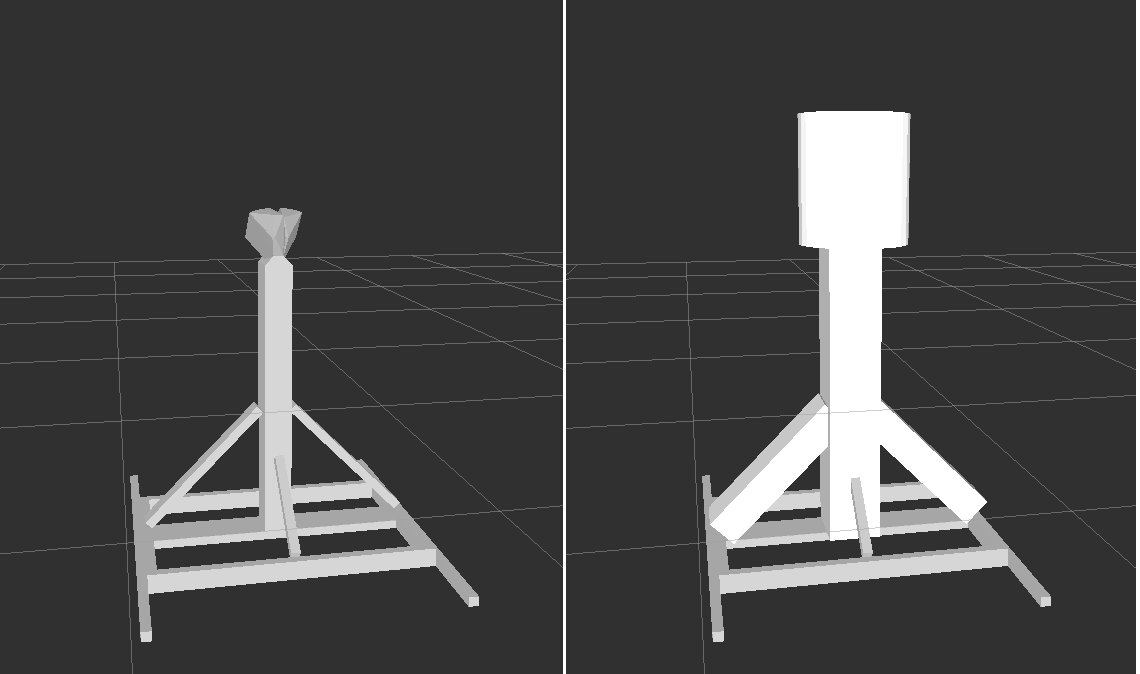
\includegraphics[width=1.0\textwidth]{images/torso.jpg}
	\caption{Left image shows visual part, right image the collidable part of the torso}
	\label{fig:torso_col}
\end{figure}
The table was modelled from primitive shapes. It was taken care that the size of the table can easily be adjusted, as can bee seen in Listing\ref{lst:table}. The collision model of the table is also slightly larger than the visual part to provide some safety margins.
\lstset{language=XML,style=customxml}
\begin{lstlisting}[caption={XML snippet, inserting the table model into the URDF}, label=lst:table]
<!-- draw the table relative to the origin -->
<xacro:model_table name="table" 
	     parent="world"
	     length="2.22"
	     width="0.8">
	<!-- Place the table relative to the world reference frame -->
	<origin xyz="-0.029 -0.3 0" />
    
</xacro:model_table>
\end{lstlisting}

When attaching the two grippers it showed that the offset between gripper wrist and last arm link was not correct. To correct that issue the file \texttt{sdh\_with\_connector.xacro} was created which simply places an additional ring between the last arm link and the gripper.\\

The file \texttt{iis\_robot\_table.xacro} draws all the pieces together. It describes the whole setup, consisting of the torso, two arms, two grippers and the table. The root element of the model hierarchy is a link called 'world\_link'. Torso, table and both arms are positioned relative to that root link. Changing the world reference frame could easily be achieved by shifting the root link to a new position. Figure\ref{fig:robot_table} shows a visualization of the URDF description.
\begin{figure}
	\centering
  	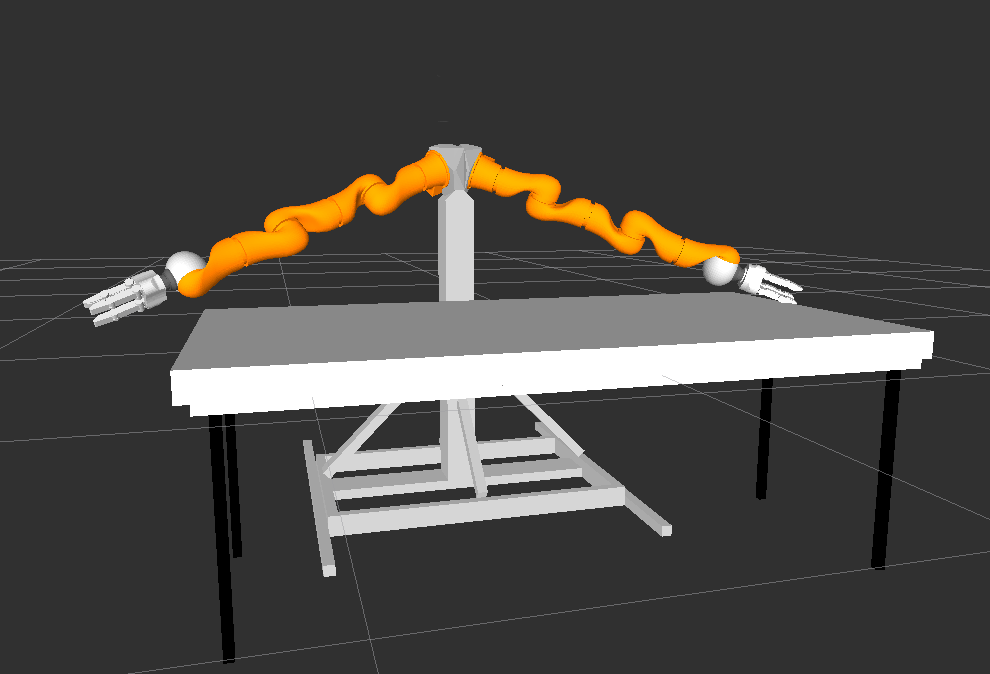
\includegraphics[width=0.75\textwidth]{images/iis_robot_table.png}
	\caption{Visualization of the URDF description}
	\label{fig:robot_table}
\end{figure}

\section{Configuring the planning tools}
\label{sec:moveit_assistant}

The MoveIt configuration package is created, using the \emph{MoveIt Setup Assistant}. Precondition is an existing URDF description of the robot setup which was created in the previous step.
The setup process comprised of the following steps:

\begin{itemize}

\item \textbf{Computation of the self collision matrix}

The self collision matrix consists of pairs of robot links that can safely be excluded from collision checking. Neighbouring links for example are in permanent collision. Collisions between other links can never happen because they are simply too far apart. The Setup Assistant calculates a large number of different robot configurations and tracks for link pairs that are mostly always in collision and pairs that are never in collision. The self collision matrix can be adjusted manually if necessary. Excluding a large number of link pairs raises performance during motion planning because collision checking is an expensive process.

\item \textbf{Defining the planning groups}

Each planning request in MoveIt is done against one of the defined \emph{planning groups}. A planning group is a group of links and joints within the model that can be seen as one logical component. Planning groups are defined for both arms and grippers. The configuration for the arms also requires the definition of the utilized IK solvers but currently only the default KDL solver is available. An additional planning group, called \texttt{both\_arms} allows planning requests for both arms simultaneously.

\item \textbf{Defining the end effectors}

End effectors are the left and the right gripper. Each end effector has a name and consists of one of the predefined planning groups, a parent group and the parent link which is the last link in the kinematic chain of the parent group.

\item \textbf{Generate the configuration files}

After completing all the configuration steps the configuration package can be generated. Therefore a target directory has to be specified which was set to \texttt{uibk\_robot\_moveit\_config}. This package is a prototype, containing a large number of predefined configuration files. Some of those files have to be extended manually, adding additional information about available robot controllers and sensors. 

\end{itemize}

Completing the last step results in a ROS package, containing necessary configuration and launch files for the given robot setup. The semantic robot description can be found in the \texttt{iis\_robot.srdf} file. It contains previously defined parameters like the self-collision matrix, planning groups and end effectors. The configuration package can be tested, running the following command on the command line:
\begin{center}
\texttt{roslaunch uibk\_robot\_moveit\_config demo.launch}
\end{center}
This command launches a \texttt{move\_group} node and a graphical user interface that can be used to test the configuration by defining planning requests. In case of a successful request, the resulting trajectories will be visualized. The setup can be modified by launching the Setup Assistant again, using the \texttt{setup\_assistant.launch} file from this package.

\section{Connecting MoveIt to the existing robot control interface}

Now MoveIt is configured and ready to handle planning requests for the IIS robot setup. This can be tested, using the 'demo.launch' file of the 'uibk\_robot\_moveit\_config' package. This starts a move\_group node, using the previously created configuration files and starts an instance of RViz together with the motion planning plugin. There it is possible to switch between the planning groups, set start and target configurations, do planning requests and visualize the outcome. But the execution of the calculated trajectories is still impossible because of the missing connection between MoveIt and the involved robot hardware. Each component needs to provide a FollowJointTrajectory action interface, defined in the 'control\_msgs' package. This is a special kind of ROS interface, designed to send trajectories to robot components and monitor the execution status. The existing control interface of the IIS robot components does not fulfil those requirements and so there had to be found a way to 'translate' those JoinTrajectory message into something compatible.

A is a set of waypoints (joint configurations). Each waypoint has to be reached at a certain time.
Those waypoints mark the important points along the path, the manipulator has to move. The controller has to be able to move the robot from point to point, satisfying the time constraints defined in the motion plan. This involves to interpolate between those trajectory points over time and calculate intermediate positions, depending on the loop rate of the control cycle. Those positions can then be sent to the robot, using the joint\_control/move topic (TODO: provide images to make that point more clear!!!). This interpolation is a difficult task and the implementation wold be far beyond the scope of this project. Luckily the required functionality is already available within the 'ros\_control' stack (wiki.ros.org/ros\_control). Those packages are created to integrate and control robot hardware in a generalized way. This facilitates the usage of existing controllers on various different robots (TODO: provide image overview of ROS control architecture and hardware adapter concept).

\subsection{Overview ROS control stack}

The infrastructure that is necessary to use the generic controllers from the 'ros\_control' packages is mainly provided by two components:

\begin{itemize}

\item \textbf{RobotHW} \\

This is the abstract base class for robot hardware abstraction. It's purpose is to send commands to the hardware and retrieves state data. Each generic controller needs a special kind of interface for controlling joints or read their current state. Concrete implementations of that class register those interfaces, based on the way how the hardware is actually controlled. For retrieving state data, a JointStateInterface is required. Controllers using that interface can query it for a specific joint and ask for the current state (position, velocity, effort). Sending commands to the joints is done via a type of the abstract JointCommandInterface, for example the JointPositionInterface which is used within this project. Other implementations are JointEffortInterface and JointVelocityInterface. Which interfaces are provided depends on the way how the concrete hardware is controlled.

\item \textbf{ControllerManager} \\

The controller manager provides a ROS interface to load, start and unload controllers and for switching between them. The control cycle is intended to run in real time
and the managed controllers are updated periodically (TODO: provide image showing the controll cycle). The main loop periodically forces the \emph{RobotHW} class to read the current state from the hardware, updates all active controllers and forces the RobotHW to send the commanded values to the hardware. This should happen in real time when interacting directly with the hardware. Controllers are usually configured on the parameter server and loaded on demand, using the ROS interface of the controller manager. Custom controllers can be created by inheriting from the abstract  \emph{ControllerBase} class.  

\end{itemize}

\subsection{Designing the hardware adapter}

The idea of the hardware adapter is to be the connection between MoveIt and the simulated or real hardware. Therefore the necessary infrastructure for using the generic controllers from the ros\_control packages has to be made available. The figure ??? gives an overview about the concept of the hardware adapter. The UibkRobotHW handles the connection to the involved robot components via their ROS interfaces. Therefore it maintains a set of JointStateAdapters, each one responsible for the communication to one robot component. A JointStateAdapter reads the current robot state from the configured 'joint\_state\_topic' and sends the commanded values to the configured 'joint\_commmand\_topic'. The adapter configuration is done via the parameter server. On startup, the hardware adapter loads the configured JointStateAdapters.

The UibkRobotHW inherits from the abstract RobotHW and represents the connection to the robot. It maintains the current state of all connected components. Therefore it maintains a set of JointStateAdapters, based on the configuration files. Each JointStateAdapter states a connection to one specific robot component. During the control cycle the JointStateAdapter reads the current joint states from the configured joint states topic and updates the received values accordingly. Commanded positions are sent to the configured joint command topic. The UIBKRobotHW also maintains a set, containing all the information about each single robot joint. The joints are identified by a unique name. During initialization, the JointStateAdapters are created, based on the adapter.config file. After creation, each JointStateAdapter waits a certain amount of time for an initial joint states message. If it does not receive such a message before timeout, it will automatically shut down for safety reasons and report an error. This is very important as the JointStateAdapter will imediately begin to send joint positions after the initialization. The position to be sent is initially the current position, as long as no other positions have been commanded by the controllers. Therefore the initial position always has to be known, otherwise dangerous and rapid robot motions could occur.

For the controllers, the UIBKRobotHW class provides a JointStatesInterface and a JointPositionInterface. The controllers will use those interfaces to access the current state and for commanding target positions.

The required configuration parameters are:

\begin{itemize}

\item \textbf{adapter\_list} \

Contains a list of all JointStatesAdapters that have to be created. For each adapter name mentioned in this list a detailed configuration is required.

\item \textbf{joint\_state\_topic} \
The name of the topic where the adapter listens for joint states. The message type of that topic has to be 'sensor\_msgs/JointStates'. This parameter is mandatory

\item \textbf{readonly} \
This parameter is optional. If true then the adapter will only listen for joint states but not publish commanded values.

\item \textbf{joint\_command\_topic} \
The name of the topic the adapter should use to publish the commanded values to. The message type, the adapter uses is 'std\_msgs/Float64MultiArray'. This parameter is necessary if the adapter is not configured to be read only.

\item \textbf{joints} \
A list of joint names that should be controlled by the adapter. The order in this list also determines the order of the values in the published message.

\item \textbf{joint\_name\_prefix} \
This parameter can be used to uniquely identify joints. For example both arms are using the same joint names (arm\_0\_joint, arm\_1\_joint,...). But the MoveIt requires joint names to be globally unique. Therefore the prefix can be used to prepend the original name to achieve uniqueness. A value of 'right\_' for example will lead to the joint names (right\_arm\_0\_joint, right\_arm\_1\_joint,...).

\end{itemize}

As the topic names, used by the JointStateAdapters can be configured, the UIBKRobotHW class is able to interact with the simulator and the real robot as well, as both of them provide exactly the same ROS interface.

During hardware adapter startup an instance of the UIBKRobotHW and ControllerManager is created from configuration. The control cycle runs in it's own thread, currently at a loop rate of 100hz. On each iteration the exact time since the last step is calculated. The ControllerManager then updates all registered controllers based on current state and time since last iteration. After handling the controllers, the JointStatesAdapters are forced to send the commanded values to the hardware. The ROS spinning and all the callback functions are handled in the original thread.



\subsection{Launching the hardware adapter}

For starting the hardware adapter, a launch file (hardware\_adapter.launch) was created in the 'uibk\_moveit\_adapter', package that handles the necessary configuration parameter upload and starts the required nodes. As it is designed to be used with the simulator and the real robot as well, it provides the 'config\_name' parameter that can be used to switch between both namespaces. Possible values are 'simulation' and 'real'. For example 'roslaunch uibk\_moveit\_adapter hardware\_adapter.launch config\_name:=real' starts the hardware adapter for the real robot. The launch file uploads the URDF robot description, the adapter and controller configuration to the parameter server. After that it runs the hardware adapter node and forces the ControllerManager to load and start the configured controllers via a ROS service call. The controller gives a lot of state information about the state and errors during the startup process. Simulator or real robot have to be launched before starting the hardware adapter, otherwise the adapter will not be able to work because of the missing initial joint states. After launching the hardware adapter, the additional controller topics can be found in the corresponding namespace, along with an additional 'joint\_states' topic that publishes the whole state of the robot at once as it is required by MoveIt.

\subsection{Adjusting the MoveIt configuration}

The prerequisites are now made for connecting MoveIt to the (simulated or real) robot. The last remaining step is to adjust the MoveIt configuration for establishing a connection to the JointTrajectoryControllers. Therefore the configuration file 'controllers.yaml' was created. It contains a list, describing the available controllers. For each controller description contains the name of the controller, it's action namespace, the type and a list, containing the names of the controlled joints.

Joint states are expected to be published via a topic named 'joint\_states'. This is done automatically by the JointStatesController.

For starting MoveIt, the launch file 'moveit\_planning\_execution.launch' was created. This file is intended to start a move\_group node either for simulated or real robot. The namespace can be selected using the boolean parameter ’simulation’. 'roslaunch uibk\_robot\_moveit\_config moveit\_planning\_execution.launch simulation:=false' starts the moveit configuration in the 'real' namespace, connecting the move\_group instance to the real robot. The launch file starts the move\_group node along with the hardware adapter and all the necessary configuration parameters. It an be chosen wether to launch it within the 'simulation' or 'real' namespace by setting the 'simulation' parameter to true or false. The launch file also starts an RViz instance configured with the motion planning plugin. This is used for visualizing the planned trajectories. It can also be used to test the connection to the robot by making a planning request and execute the resulting trajectory.


\section{Usage examples} 

\subsection{Capabilities}

\subsection{Modifying the planning scene}

\subsection{Planning and executing trajectories}

\subsection{Running the planning tools in different namespaces}
How to use MoveIt with the simulator or real robot in parallel